\section{Proposition d'une nouvelle solution}
\subsection{Gestion de l'inventaire matériel}
La première étape consiste à créer une base de données exhaustive de tous les équipements 
qui nécessitent une maintenance. Chaque équipement doit être enregistré avec des 
informations telles que le nom, le modèle, le numéro de série, la date d'installation, 
les caractéristiques techniques, etc.
\subsection{Planification des activités de maintenance}
Une fois que l'inventaire des équipements est établi, les activités de maintenance 
préventive et corrective doivent être planifiées. La GMAO permet de créer des 
calendriers de maintenance régulière pour chaque équipement en fonction des 
recommandations du fabricant, des normes industrielles ou des exigences spécifiques 
de l'entreprise.
\subsection{Gestion des interventions}
Lorsqu'une intervention de maintenance est nécessaire sur un équipement, une demande 
d'intervention est générée dans la GMAO. Cette demande est ensuite assignée à un 
technicien ou une équipe de maintenance appropriée.
\subsection{Suivi des interventions}
Les techniciens utilisent la GMAO pour enregistrer les détails de chaque intervention 
effectuée sur un équipement. Cela inclut les actions entreprises, les pièces de 
rechange utilisées, le temps passé sur l'intervention, etc.
\subsection{Historique des matériels}
La GMAO conserve un historique complet de toutes les interventions et activités de
 maintenance effectuées sur chaque matériel. Cela permet d'analyser les 
 tendances de défaillance, de prévoir les besoins futurs en maintenance et 
 d'optimiser les processus.
\subsection{Indicateurs de performance}
Une GMAO peut fournir des rapports et des tableaux de bord pour suivre les indicateurs 
de performance clés (KPI) liés à la maintenance des équipements. Ces KPI peuvent 
inclure le taux de disponibilité des équipements, le temps moyen entre les défaillances, 
le taux de réussite des interventions, etc.

\subsection{Conception de base de données}
Pour bien comprendre ce qui a été fait et savoir d’où je dois partir, il m’a fallu 
analyser les différentes tables présentes en base de données. 

Pour mettre au propre cette partie, j’ai modélisé un diagramme d’entité association 
qui reprend partiellement les tables de l’ancien module GMAO. J’ai réalisé seulement 
une portion du diagramme d’entité association puisque le module GMAO contient beaucoup 
de tables dont un certain nombre qui ne concernent pas les évolutions que je dois y 
apporter. 

De plus, le diagramme n’est pas complet. J’ai donc reproduit le diagramme d’entité 
association uniquement pour la partie qui concerne la mise en place de la gestion de 
l’inventaire matériel. 

L'objectif de ce projet est de fournir un système destiné à gérer le parc matériels des 
laboratoires médicaux. Ce système fait partie de l’application MCA. Il est accessible 
via un navigateur. 

Le module permet d'avoir une vue globale sur le parc matériels, de gérer et de contrôler 
le travail des techniciens sur le terrain tout en centralisant les informations sur les 
matériels se trouvant dans les différents sites de laboratoire. 

Le module permet aux techniciens sur le terrain de renseigner leurs activités, d'avoir 
les informations sur les matériels et aux usagers de déclarer les pannes.
\begin{figure}[hp]
    \centering
    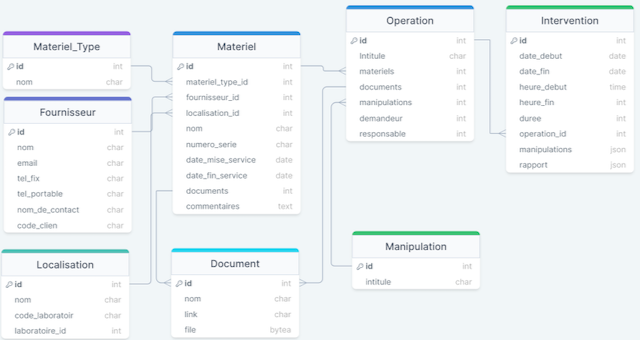
\includegraphics[width=400pt]{images/db_diagramm.png}
    \caption{Modèle entité-association de la solution GMAO}
\end{figure}
\pagebreak

Les matériels sont attachés à un type pour faciliter le filtrage et pour regrouper les 
différents matériels à une famille de type. Les informations des fournisseurs sont 
aussi attachées aux matériels.

 Les agents de maintenance peuvent planifier plusieurs maintenances en même temps, 
 ainsi, ils peuvent intervenir sur plusieurs maintenances et générer les rapports 
 d’interventions.

Aussi, il est possible de télécharger plusieurs fichiers qui seront utiles au moment 
de la maintenance : guide d’utilisation de matériel, documentation technique de 
constructeur, etc.

Dans le module GMAO, les techniciens de laboratoire pourront ajouter, modifier ou 
supprimer des matériels. 

Il faudra développer une interface composée d’un tableau qui reprend tous les 
matériels enregistrés en base de données en indiquant leur type, leur fournisseur 
et les documents associés. 

De cette manière, les utilisateurs verront rapidement l’état de l’inventaire matériel 
et toutes les informations associées.

Une fois que cette gestion de l’inventaire sera correctement implémentée dans le 
module GMAO, il me faudra adapter la fonctionnalité de la maintenance. En effet, 
lors d’une demande de maintenance sur un matériel géré dans le module GMAO, 
l’utilisateur devra être capable d’indiquer l’indisponibilité de ce matériel sur 
lequel la maintenance sera effectuée.
\pagebreak